\documentclass[12pt, oneside]{article}
\usepackage[letterpaper, margin=1in, headsep=0.5in]{geometry}
\usepackage[english]{babel}
\usepackage[utf8]{inputenc}
\usepackage{amsmath}
\usepackage{amsfonts}
\usepackage{amssymb}
\usepackage{tikz}
\usetikzlibrary{quotes, angles}
\usepackage{graphicx}
%\usepackage{pgfplots}
%\pgfplotsset{width=10cm,compat=1.9}
%\usepgfplotslibrary{statistics}
%\usepackage{pgfplotstable}
%\usepackage{tkz-fct}
%\usepackage{venndiagram}

\usepackage{fancyhdr}
\pagestyle{fancy}
\fancyhf{}
\rhead{\thepage \\Name: \hspace{1.5in}.\\}
\lhead{BECA / Dr. Huson / 11.1 IB Math\\* Unit 1: Algebra Review}

\renewcommand{\headrulewidth}{0pt}


\begin{document}

\subsubsection*{Quadratic functions: solve for the roots or zeros of the function, $f(x)=0$}

For each function, first factor it (always show this step), then state the roots using the form, ``$x=3,4$'' (or whatever the values are).

\begin{enumerate}

\item   $f(x)=x^2+7x+12$\\*[60pt]
\item   $f(x)=x^2+13x+12$\\*[60pt]
\item   $f(x)=x^2-4x-12$\\*[60pt]
\item   $f(x)=2x^2-10x-12$\\*[60pt]
\item   $f(x)=-3x^2+6x-3$\\*[60pt]
\item   $f(x)=\frac{1}{2}x^2+2x+2$\\*[60pt]

\newpage
\subsubsection*{Model situations with quadratic functions}
\item Expand from vertex form to standard form, $ax^2+bx+c \text{ where } a, b, c \quad  \epsilon R$
\begin{enumerate}
  \item   $f(x)=(x-2)^2+6$
  \item   $f(x)=(x-5)^2-9$
\end{enumerate}

\item Factor each function.
\begin{enumerate}
\item   $f(x)=x^2+5x+6$
\item   $f(x)=x^2-7x+10$
\item   $f(x)=x^2+6x+8$
\item   $f(x)=x^2-2x-8$
\item   $f(x)=x^2-7x-8$
\item   $f(x)=x^2+3x-10$
\end{enumerate}

\subsubsection*{Completing the square}

Rewrite the function in vertex form, $f(x)=(x-h)^2+k$. Include the step showing the $(-\frac{b}{2a})^2$ term.
\item   $f(x)=x^2-6x+11$
\vspace{3cm}
\item   $f(x)=x^2+8x+9$
\vspace{3cm}

Expand the function from vertex form to standard form, $ax^2+bx+c \text{ where } a, b, c \;  \epsilon \; \mathbb{R}$. Then factor the result and state the roots. Sketch the function, labeling the intercepts with values and the vertex as an ordered pair.
\item   $f(x)=(x-2)^2-9$
  \begin{flushright} %4 quadrant regents grid
  \begin{tikzpicture}[scale=0.35]%[scale=0.635]
    %\draw [help lines] (-10,-10) grid (10,10);
    \draw [thick, ->] (-10.2,0) -- (10.4,0) node [below right] {$x$};
    \draw [thick, ->] (0,-10.2)--(0,10.4) node [left] {$y$};
  \end{tikzpicture}
  \end{flushright}

\newpage
\subsubsection*{Graphing quadratics}
\item Graph the function $f(x)=-x^2-4x+5$. You may use a graphing calculator rather than factoring the function and completing the square.\\*[5pt]
Label the scales with at least a few values. Mark the vertex as an ordered pair and label each intercept with its value.\\

\begin{center} %4 quadrant regents grid
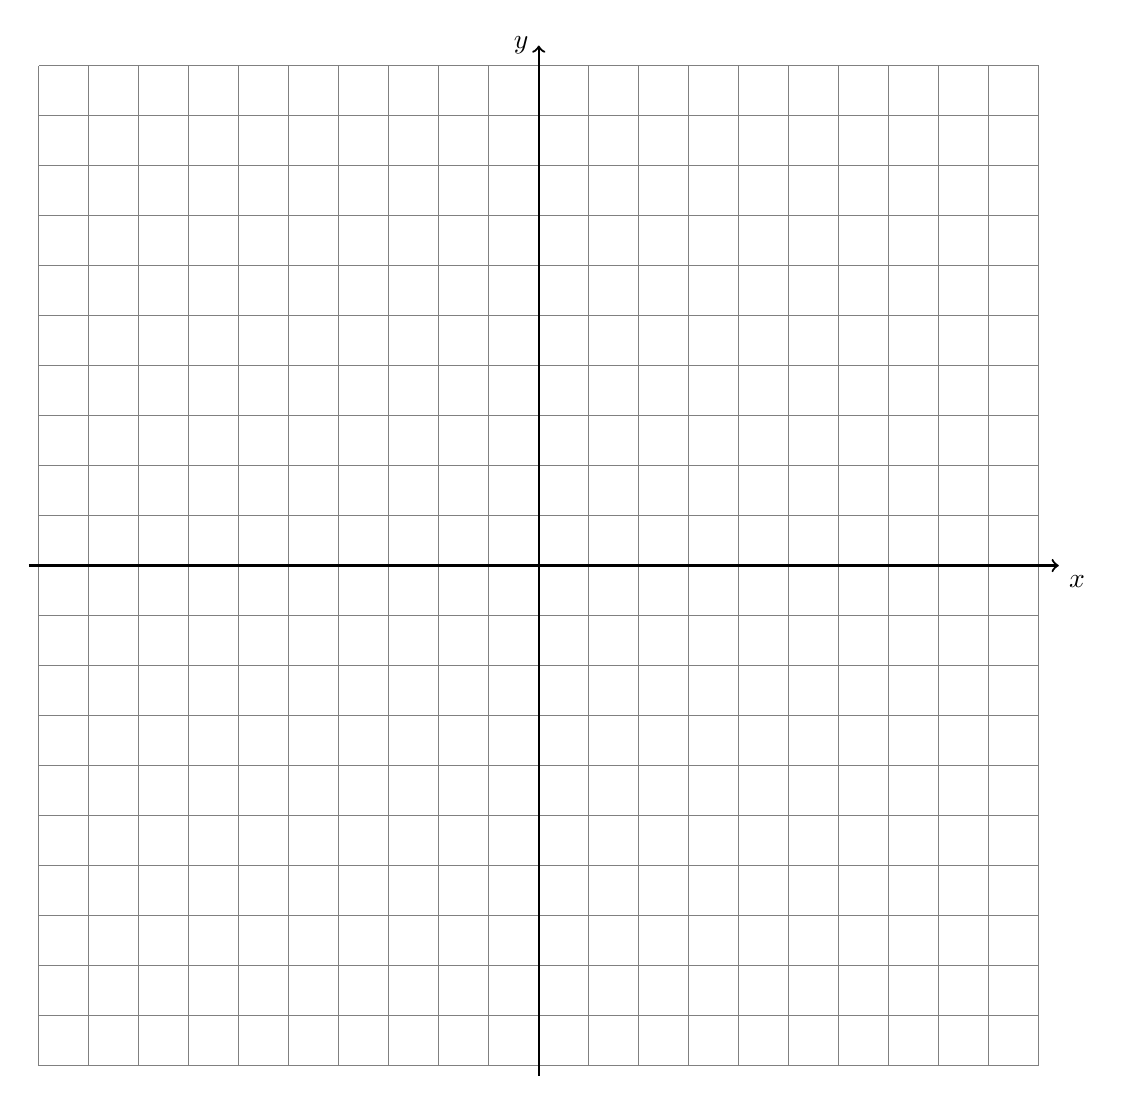
\begin{tikzpicture}[scale=0.635]%[scale=0.635]
  \draw [help lines] (-10,-10) grid (10,10);
  \draw [thick, ->] (-10.2,0) -- (10.4,0) node [below right] {$x$};
  \draw [thick, ->] (0,-10.2)--(0,10.4) node [left] {$y$};
\end{tikzpicture}
\end{center}

\newpage
\subsubsection*{Model situations with quadratic functions}

Use a graphing calculator to view the graph and a table of values for the following function:
\[h(x)=-\frac{1}{225}x^2+\frac{2}{3}x\]
where $h(x)$ represents the height of an object and $x$ it's horizontal position.\\*[5pt]
Make a table of values to the left of the graph, below. Include key values. Graph the function over domain where $h(x) \geq 0$. Use a horizontal scale of 1 square equals 10 units and vertical scale of 1 square equals 2.5 units. Label the intercepts and vertex.\\*[30pt]

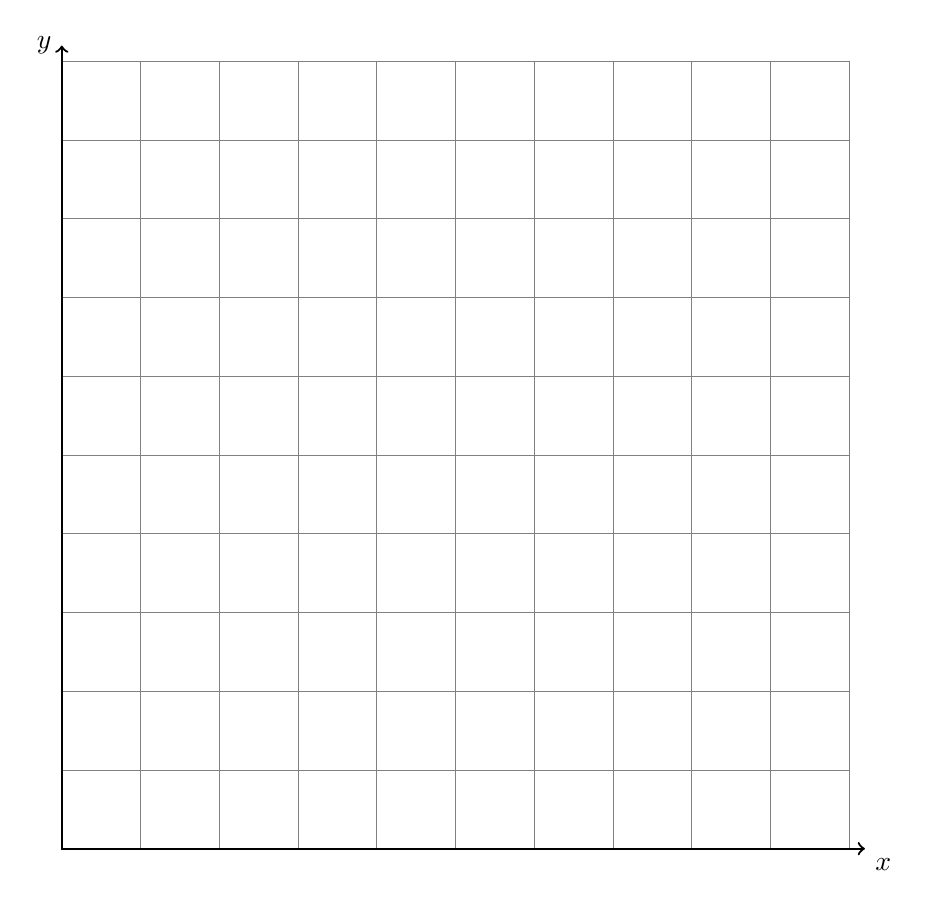
\begin{tikzpicture}%[scale=0.8]
  \draw [help lines] (0,0) grid (10,10);
  \draw [thick, <->] (0,10.2) node [left] {$y$}
       -- (0,0) -- (10.2,0) node [below right] {$x$};
\end{tikzpicture}

\subsection*{The inverse of a function}
Derive the inverse of each function. Simplify the expression.
\item   $f(x)=\frac{1}{2}x+2$
\item   $f(x)=\frac{2}{3}x^2-3$
\item   $f(x)=\sqrt{x-1}+\frac{1}{2}$

\subsection*{Function substitution}
\item Given $f(x)=x^2-1$. Simplify $f(2x-1)$?
\item Given $f(x)=x^3$. Simplify $f(x+1)$?
\item Given $f(x)=4-(2x^2+x)$. Simplify $f(\frac{1}{2}x-3)$?

\subsection*{Function composition}
In each exercise, perform the composition $f \circ g$ and simplify.
\item Given $f(x)=\frac{1}{2}x^2+1$ and $g(x)=2x$
\item Given $f(x)=\sqrt{x-4}$ and $g(x)=x^2+4$
\item Given $\displaystyle f(x)=\frac{1-x}{x^2}+1$ and $g(x)=2x+3$

\item Given $f(x)=3x+2$. What is the inverse of the function $f^{-1} (x)$?

\begin{enumerate}
    \item Rewrite the function reversing $x$ and $y$. (assume that $y$ and $f(x)$ are interchangeable)\\*[20pt]
    \item Solve for $x$. Finish by putting $y$ on the left side of the equality.\\*[60pt]
    \item State the answer as $f^{-1} (x)$ equals an expression.\\*[15pt]
\end{enumerate}

\subsection*{Function substitution}
\item Given $f(x)=3x+2$. What is $f(2x-1)$?
\begin{enumerate}
    \item Perform the substitution, putting $2x-1$ in parenthesis.\\*[20pt]
    \item Simplify, beginning each line with a leading equals sign if it is equal to the line above.\\*[40pt]
\end{enumerate}

\subsection*{Function composition}
\item Given $f(x)=x^2+2$ and $g(x)=x^2$ What is $(f \circ g)(x)$?\\*
\begin{enumerate}
    \item Rewrite $f \circ g$ and perform the inner substitution (i.e. for $g$): $f(g(x))=f(x^2)$\\*[20pt]
    \item Perform the substitution, putting $x^2$ in parenthesis (and using a leading equals sign).\\*[20pt]
    \item Simplify, beginning each line with a leading equals sign.\\*[20pt]
\end{enumerate}

\end{enumerate}
\end{document}
